\section{3D pose estimation}
From a historical perspective, a 3d motion capture algorithm consists of 4 sequential processes: initialisation, tracking, pose estimation and recognition. Initialization involves both camera and model initialization, i.e. setting the camera calibration and finding a model that represents the subject and assigning its initial pose manually or automatically. Model-based approaches can be viewed iteratively, with each frame of the data source representing an iteration in which the initial pose is refined. Tracking is concerned with the relationship between the parts of the subject's body. This leads to segmentation of the subject from the background, representation changes, and establishing tracking in further images. The next phase, which is mainly covered in this section, is the estimation of the pose. A distinction is made between model-based and non-model-based methods, with the former requiring  \emph{a priori} a model. In that approaches, especially human pose estimation, a human model is used to benefit from its encoded information. This model can either be used indirectly, considering e.g. only general aspects such as size and structure, or it is a direct used model. Directly used models are both more detailed and offer broader benefits in regards to occlusion handling and embedded kinematic constraints. In an application, the observed object is approximated by the model, which is continuously refined with further images.\cite{summary80s}
\\
As with 2D Pose Estimation, neural networks, particularly convolutional networks, have successfully been used to achieve more accurate results than earlier methods \cite{WANG2021103225, Chen2016, Chen_2017_CVPR, Tome_2017_CVPR, Andrikula2010, Ye2011, Martinez_2017_ICCV}. Since neural networks can be very resource intensive to compute and the architecture can be extremely complex when working with 3D data, many  of the presented approaches use 2D Pose Estimation followed by an uplifting process to 3 dimensions. Also, a lot of 2D training data is available in comparison to 3D data which could be used to train a neural network, because the annotation process is way harder in higher dimensions. Therefore \cite{Chen2016} presents a process to synthesize training images and shows that neural networks training with data generated by their method are even more effective than neural networks which were trained using real images. \cite{Rogez2016} presents a similar approach.

\subsection{Lifting from 2D to 3D pose}
For uplifting, recent work has proven statistical models such as (deep) neural networks themselves \cite{Tome_2017_CVPR, Martinez_2017_ICCV}, matching the estimated 2D pose with a database \cite{Chen_2017_CVPR} or triangulation using multiple viewpoints \cite{Dong_2019_CVPR} useful. In particular \cite{Martinez_2017_ICCV} shows that even very simple deep neural networks can be extraordinarily effective for uplifting 2D to 3D pose estimations, considering both computational resources and failure rate.
\newline
Inspired by various 2D human pose estimation algorithms, many studies have employed the outputs of 2D pose estimate methods for 3D human pose estimation to improve in-the-wild generalization performance. For example, Martinez et al. \cite{Martinez_2017_ICCV} pioneered the research on lifting 2D poses to 3D space with a simple yet effective neural network. Other methods \cite{park_3d_2016, wang_deep_2021, zhou_hemlets_2019, habibie_wild_2019, tekin_learning_2017} focus on fusing 2D joint heat maps from the top-down 2D pose estimation methods with 3D image cues to reduce ambiguity. 

\begin{figure*}[!htb]
	\centering
	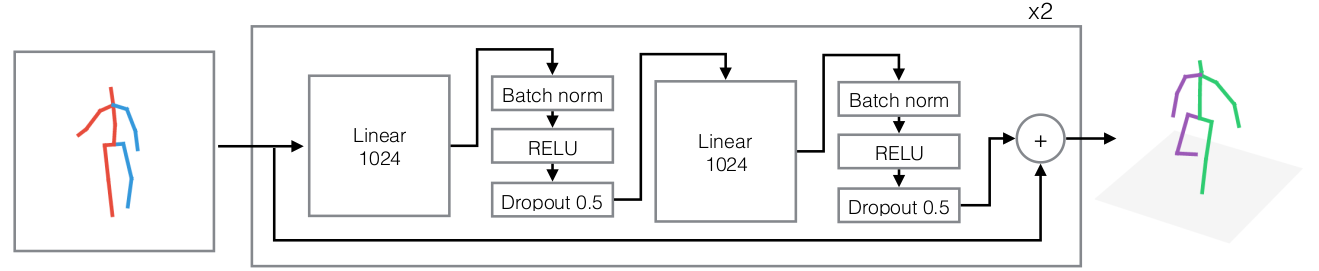
\includegraphics[scale=0.4]{3dpose/martinez_network.png}
	\caption{Neural network structure from \cite{Martinez_2017_ICCV}}
	\label{fig:martinez_network}
\end{figure*}

\begin{figure*}[!htb]
	\centering
	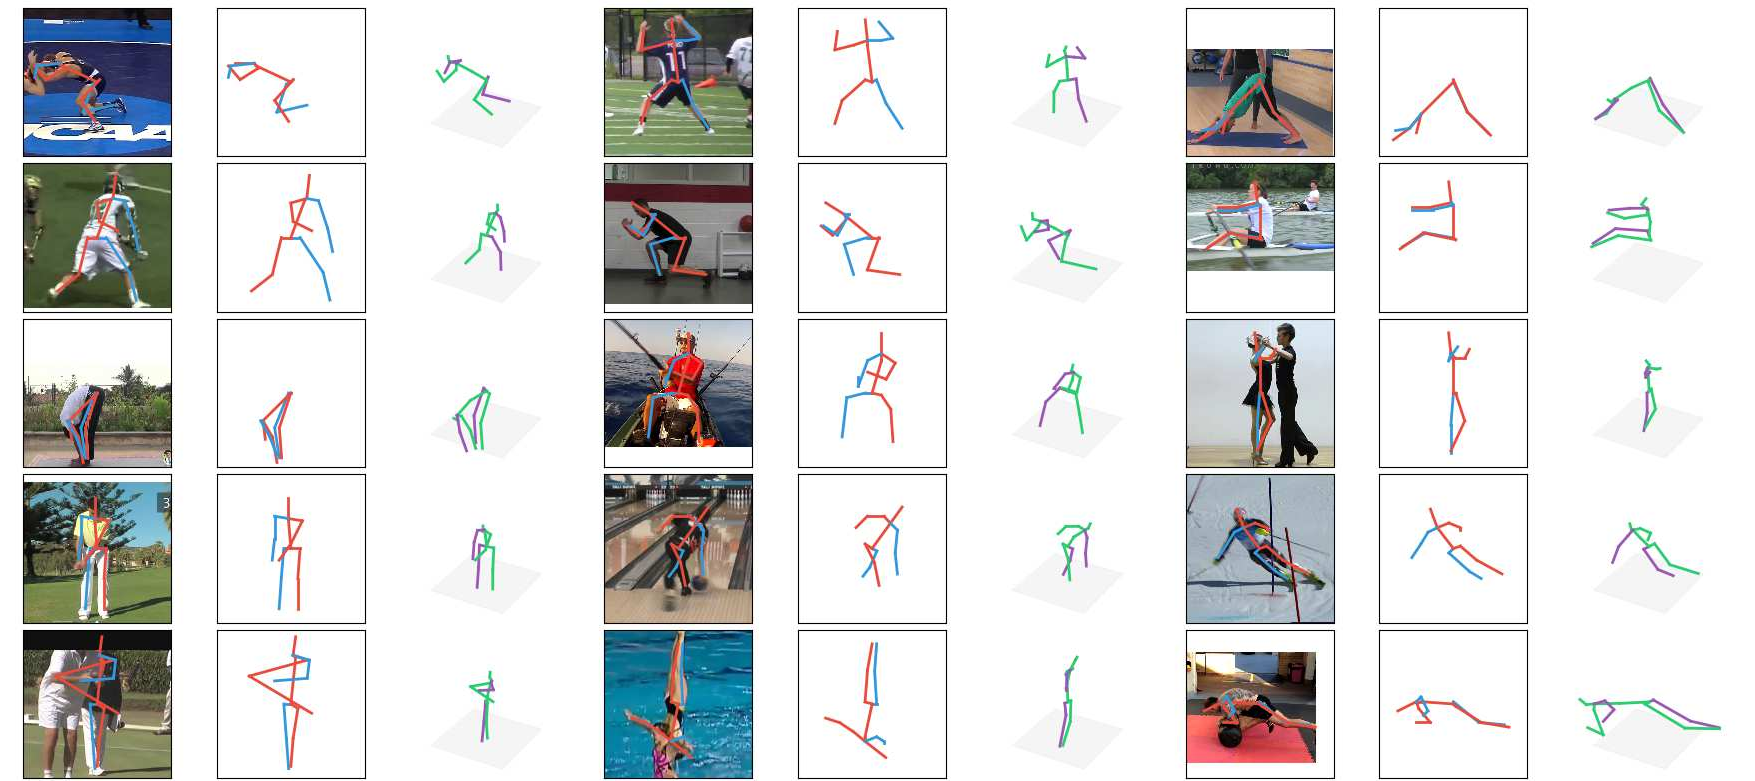
\includegraphics[scale=0.3]{3dpose/martinez_test_cases.png}
	\caption{Test cases from \cite{Martinez_2017_ICCV}}
	\label{fig:martinez_test_cases}
\end{figure*}

\subsubsection{A simple yet effective baseline for 3d human pose estimation}
While trying to investigate common errors in the uplifting process, \cite{Martinez_2017_ICCV} created a method with state-of-the-art results for 3d pose estimation using a very basic neural network with recently proposed optimization methods, whose structure is shown in \autoref{fig:martinez_network}. Linear layers changing the input and output dimensions are not shown. 2d joint positions are used as input data determined by the so called stacked hourglass network as described in \cite{Newell2016}, while the output consists of 3d joint positions.\\
 Since the 2d joint positions are low-dimensional and therefore no highly complex computation is necessary, a simple linear layer with a RELU activation function is used first, followed by batch normalization and dropout as presented in \cite{srivastava2014} to prevent overfitting and improve result quality at the cost of a slight increase in computation time during training and testing. This structure is then repeated and a residual connection to the output added. These connections are proposed to help improve performance, reduce training time and lower error rates in \cite{HeZRS15}. The whole network established so far is doubled to complete the architecture which in sum consists of 4 to 5 million trainable parameters. It was then trained on Human3.6M, a dataset with 3.6 million 3d poses of humans during normal activities such as eating or walking \cite{H3.6M}.\\ Testing results show that this approach outperformed previous methods like \cite{PavlakosZDD16} in most cases, despite the simple architecture that was used. However, testing on the MPII Human Pose Dataset \cite{andriluka14cvpr} also revealed limitations of the network shown especially in the bottom row of \autoref{fig:martinez_test_cases}. Firstly (left and right picture), the 2d joint position must be detected properly. The middle picture also rendered a problem, which according to the original paper comes down to poses being not included in the Human3.6M dataset, such as upside-down poses or examples not showing a full human body.\\
 The authors conclude that basic neural networks today are already able to produce very good results in terms of accuracy for uplifting 2d to 3d human poses. Therefore one of the main error sources of this process remains 2d pose estimation and more complex models should be able to perform the task of uplifting even better.
 
\subsection{3d pose directly from 2d image}
currently way worse than uplifting, maybe not write a lot here
\subsection{Direct 3d pose estimation}
Methods working directly on 3D data, such as \cite{Ye2011} (working with depth maps) can avoid potential sources of error such as projections or lighting conditions. This leads to more robust and accurate results, however more complex (neural network) architectures and computational resources are required. Traditional methods like the least-squares-estimation presented in \cite{Haralick98} work without training data needed and are computationally inexpensive, but yield rather high error rates compared to newer methods.

\subsubsection{Skinned Multi-Person Linear model SMPL}
In \emph{SMPL} a model $M(\vec{\beta},\vec{\theta},\phi)$ is learned from the 3d scans explained in \autoref{sec:benchmarks}, that returns a mesh from the input. This formulation is also included in \autoref{eq:model}, where $\mathbb{R}^{3N}$ is a vector of \emph{N = 6890} vertices sculpturing the mesh. In this formula, $\vec{\beta}$ is a vector of blend shapes, while $\vec{\theta}$ are poses and $\phi$ describes the displacement of soft tissues.

\begin{equation}
\label{eq:model}
M(\vec{\beta},\vec{\theta},\phi) : \mathbb{R}^{\vert \vec{\theta} \vert \times \vert \vec{\beta} \vert} \mapsto \mathbb{R}^{3N}
\end{equation}

\emph{SMPL} is based on vertex skinning and blend shapes. A vertex changes its position depending on the motion of the associated joint. This displacement is controlled by assigned blend weights. A vector $T \in \mathbb{R}^{3N}$ of vertex positions describes a gender neutral initial human model, while a matrix $W \in \mathbb{R}^{N \times K}$ represents the blend weights per vertices and \emph{K = 23} joints. The joints that describe the human structure and form the skeleton are represented by rotation vectors. Moreover, T can be rearranged by the pose-blending function $B_{P}(\vec{\theta})$ according to the given poses, leaving T unaffected, while $B_{S}(\vec{\beta})$ reshapes the identity model by its given shape blends.

\cite{smpl}

